\documentclass[4paper]{article}
\usepackage{fullpage,graphicx}
\begin{document}
\section{Hardware modifications}

The default Redpitaya STEM-lab (14-bit) configuration is to route the
unbalanced SMA input (high-impedance) through a differential
amplifier LTC6403-1 acting also as a low pass filter feeding the ADC with 
a differential input. In order to allow for undersampling since the LTC2145
ADC input track and hold allows for a much broader bandwidth than
half the sampling rate, the following connections must be performed:
\begin{itemize}
\item for each channel, remove the inductor (black component) between the
differential output of the amplifier and the ADC. Solder the output of the balun
to the pads connected to the ADC (red circles, channels 1 and 2),

\begin{center}
\begin{minipage}[t]{\linewidth}
\begin{minipage}{.45\linewidth}
\includegraphics[width=\linewidth]{../DSC_0526.JPG}
\end{minipage}
\begin{minipage}{.46\linewidth}
\includegraphics[angle=180,width=\linewidth]{../DSC_0528.JPG}
\end{minipage}
\end{minipage}
\end{center}

\item for each channel, connect the reference voltage to the center point of each
balun output (blue circles, channels 1 and 2)
\end{itemize}

The test setup is as follows: an ARE quartz oscillator (13~dBm output) feeds the
clock input of the ADC. The ouput of an Ettus Research B210 generates a signal
between 50 and 875~MHz sampled by one channel, while the second channel is loaded by
a 50~$\Omega$ reference resistance to assess crosstalk:

\includegraphics[width=\linewidth]{../DSC_0527.JPG}

The bitstream for recording the measurements has been slightly modified
to probe both inputs (ADC A and B) and feed the DMA stream with both inputs:

{\footnotesize
\begin{verbatim}
set_property -dict [list CONFIG.PCW_IRQ_F2P_INTR 1 CONFIG.PCW_USE_FABRIC_INTERRUPT {1} CONFIG.PCW_USE_S_AXI_HP0 {1}] $ps7

add_ip_and_conf redpitaya_converters converters { DAC_EN false ADC_SIZE 14 }

connect_proc_rst converters adc_rst_i
connect_to_fpga_pins converters phys_interface phys_interface_0
connect_intf converters clk_o ps7 S_AXI_HP0_ACLK

add_ip_and_conf dataReal_dma_direct dataReal {NB_INPUT 2 NB_SAMPLE 500000 \
SIGNED_FORMAT true DATA_SIZE 14 USE_SOF false STOP_ON_EOF false }

connect_intf converters dataA_out dataReal data1_in
connect_intf converters dataB_out dataReal data2_in
connect_intf converters clk_o dataReal m00_axis_aclk
connect_proc dataReal s00_axi 0x1000

add_ip_and_conf axi_dma axi_dma_x {c_include_sg false c_sg_length_width 24 c_include_mm2s false c_s2mm_burst_size 32}

connect_intf dataReal m00_axis axi_dma_x s_axis_s2mm
connect_intf axi_dma_x s2mm_introut ps7 irq_f2p

apply_bd_automation -rule xilinx.com:bd_rule:axi4 -config {Master "/ps7/M_AXI_GP0" Clk "Auto" } \
    [get_bd_intf_pins axi_dma_x/s_axi_lite]
apply_bd_automation -rule xilinx.com:bd_rule:axi4 -config {Master "/axi_dma_x/M_AXI_S2MM" Clk "Auto"} \
    [get_bd_intf_pins ps7/s_axi_hp0]

connect_bd_net [get_bd_pins rst_converters_125M/peripheral_reset] [get_bd_pins dataReal/m00_axis_reset]
save_bd_design
\end{verbatim}
}

Measurements for various frequencies well above half the sampling frequency have been collected
and are displayed below

\vspace{-0.3cm}
\begin{center}
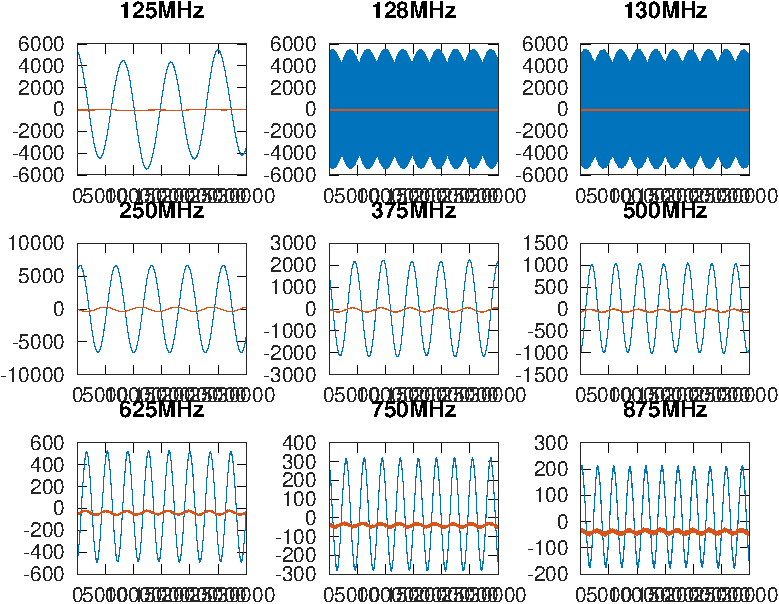
\includegraphics[width=.8\linewidth]{all}
\end{center}

For each chart, the signal drives the blue curve and the red curve is the loaded ADC input which 
should, if perfectly isolated, not display any voltage variation. The signal frequencies are, except
for 128 and 130~MHz, multiples of the 125~MHz sampling frequency. The beatnote is the frequency
difference between the ARE oscillator and the B210 reference oscillator.
\end{document}
